%! TeX root = master.tex
% !TEX program = lualatex
\lecture{6}{24-03-2026}{Overfitting, Cross-validation and Regularization}{}
\subsection{Model complexity}
When using non linear model we should care about the model complexity, because by using those type of model
 we have added flexibility, that can make the model too complex fot the task at hand. 

\textbf{E.g,} a high degree polynomial is more complex than a low degree one.

\subsection{Overfitting vs Underfitting}
\textbf{Overfitting:} when the error on the test data is larger than the training data. 

\textbf{Underfitting:} when the error is large on $both$ training and test data. 

The general phenomenon look like this:

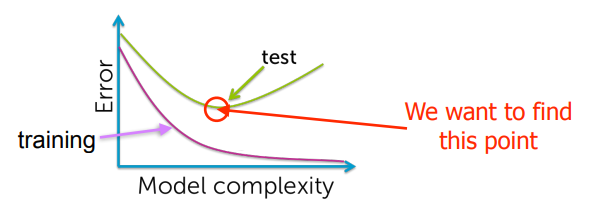
\includegraphics[width=0.5\linewidth]{images/img_20260324_090839.png}

Thus we want to find the point that minimize the test data error (model selection), without having prior access to the test data. 

To do that we could use \textbf{Cross-validation}.

\subsection{Cross-validation}
First let's start with an example of a regression problem with 1D input x, 1D output y, 
and let's consider 3 different models of increasing complexity:

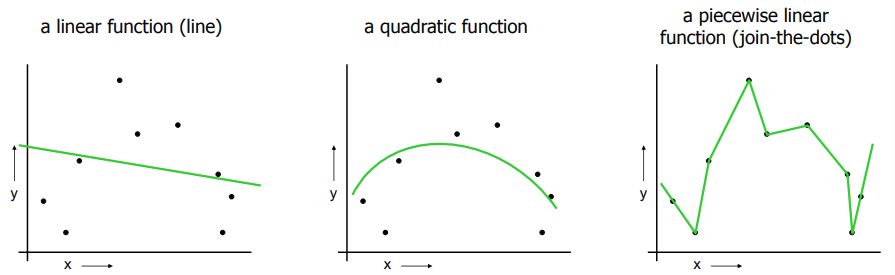
\includegraphics[width=0.8\linewidth]{images/img_20260324_091416.png}

Here the best models is the quadratic function, because we have non prior knowledge of the test data (only the same distribution), hence 
the piecewise linear function will probably work poorly on it (it is an overfitted model as it goes through each point of the training set but it is completely wrong between those points).
\newpage
\subsubsection{The validation set method}

\begin{enumerate}
  \item Randomly choose, e.g., 30\% of the data to form a \textcolor{red}{validation set}
  \item The remainder then acts as your new \textcolor{blue}{training set}

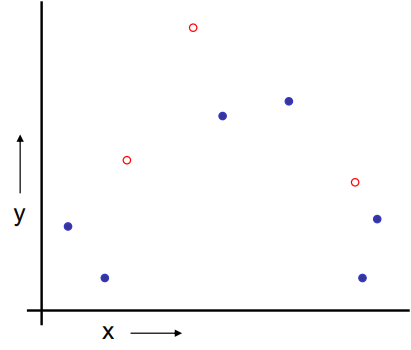
\includegraphics[width=0.3\linewidth]{images/img_20260324_095608.png}
  \item Perform regression on this new training set only


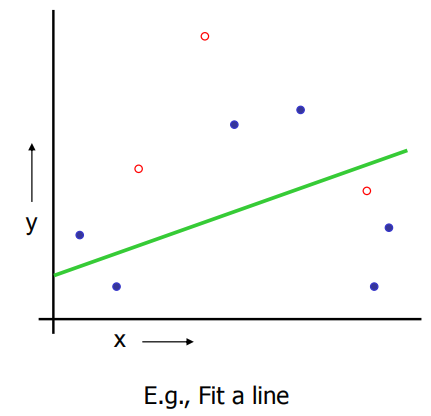
\includegraphics[width=0.3\linewidth]{images/img_20260324_100140.png}
  \item Estimate the performance on the test data using the validation set

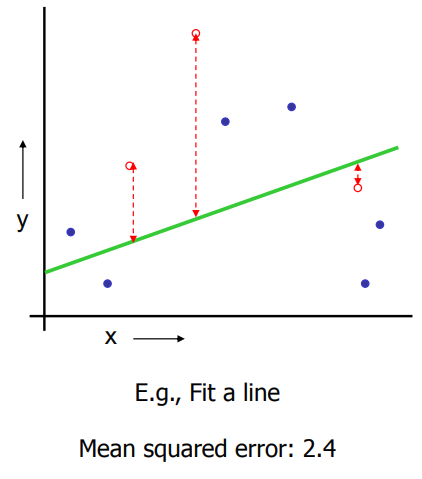
\includegraphics[width=0.3\linewidth]{images/img_20260324_100345.png}
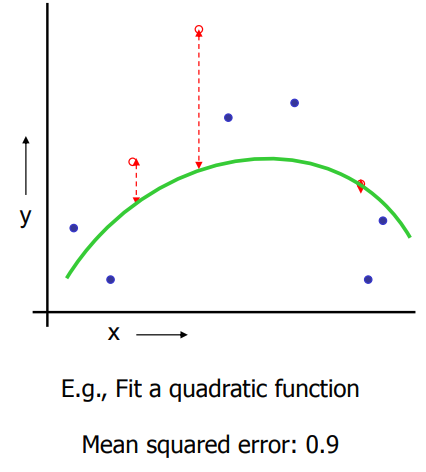
\includegraphics[width=0.3\linewidth]{images/img_20260324_100303.png}
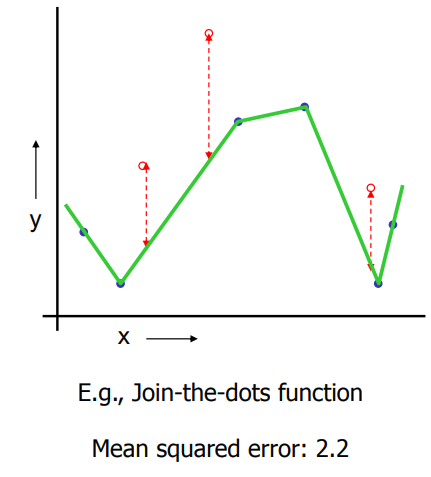
\includegraphics[width=0.3\linewidth]{images/img_20260324_100317.png}
\end{enumerate}

\textbf{Upsides:}
\begin{itemize}
  \item Very simple
  \item We can choose the model based on the validation error
\end{itemize}
\textbf{Downside:} Unreliable estimate of future performance. 

\subsubsection{Leave-one-out cross-validation (LOOCV)}
\begin{enumerate}
  For $i = 1, \dots, N$
  
  \item Let \textcolor{red}{$(x_i, y_i)$ be the $i^{th}$ sample}

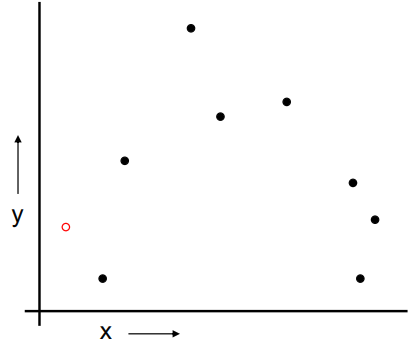
\includegraphics[width=0.3\linewidth]{images/img_20260324_100818.png}
\item Temporarily remove \textcolor{red}{$(x_i, y_i)$} from the training set 
  \item Perform regression on the remaining $N-1$ samples (e.g., fit a line)
  \item Compute the error on \textcolor{red}{$(x_i, y_i)$} 

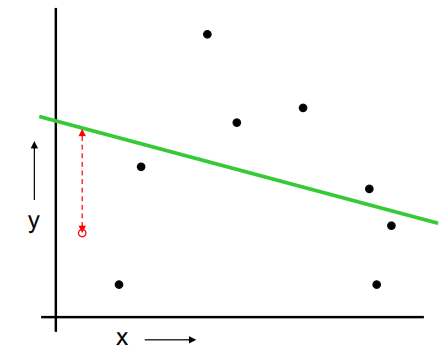
\includegraphics[width=0.3\linewidth]{images/img_20260324_101018.png}
\end{enumerate}
When you have done all points, report the average error.


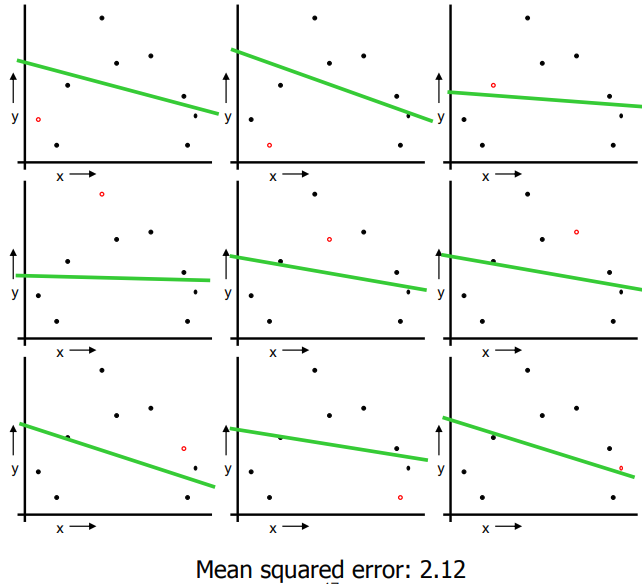
\includegraphics[width=0.33\linewidth]{images/img_20260324_101135.png}
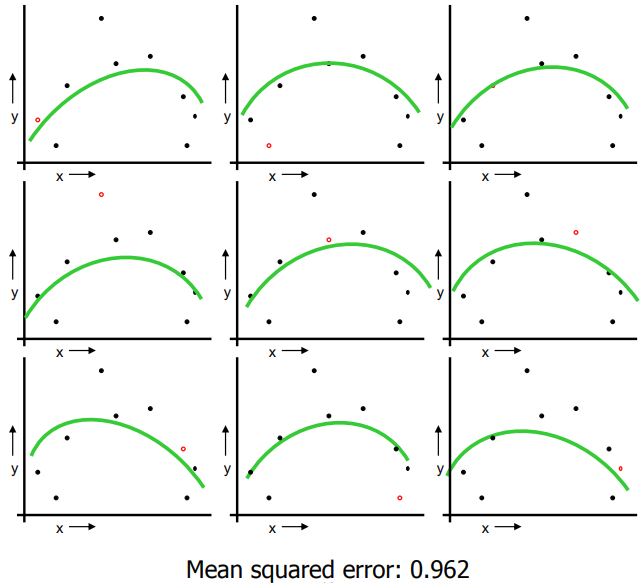
\includegraphics[width=0.33\linewidth]{images/img_20260324_101159.png}
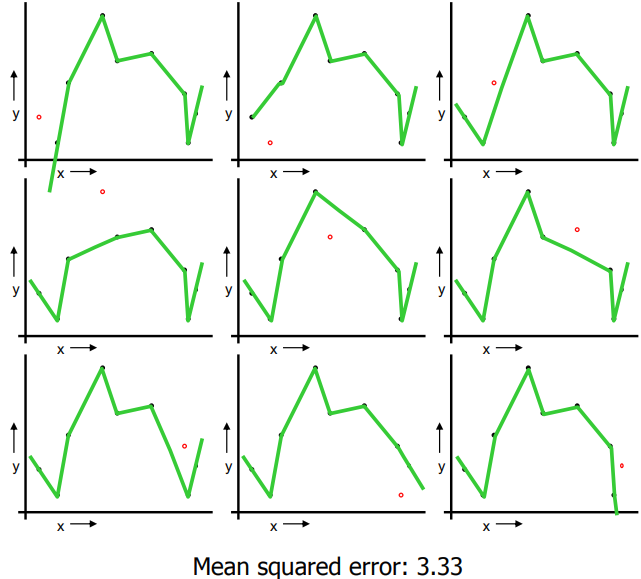
\includegraphics[width=0.33\linewidth]{images/img_20260324_101221.png}

\textbf{Upside:} Doesn't waste data

\textbf{Downside:} Expensive

\subsubsection{$k$-fold cross-validation}

Randomly split the dataset into $k$ partitions (e.g., $k = 3$, shown with different colors)

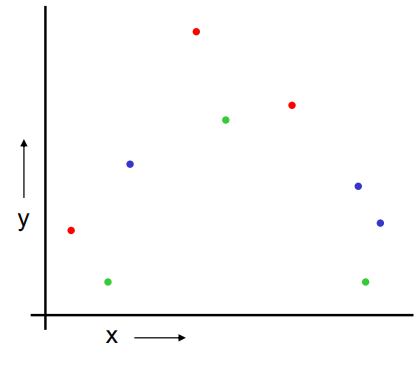
\includegraphics[width=0.3\linewidth]{images/img_20260324_102101.png}
\begin{itemize}
\item For the \textcolor{red}{red} partition, train on all the points \textbf{not} in the red partition. Compute the errors on the red points (e.g, with a line). 

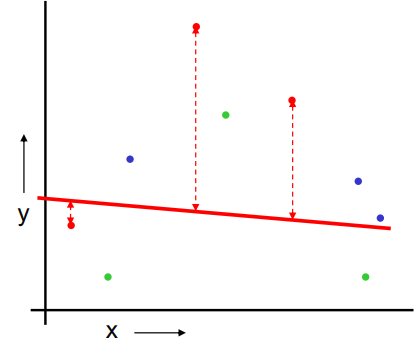
\includegraphics[width=0.3\linewidth]{images/img_20260324_102324.png}
\item Same for the \textcolor{green}{green} and the \textcolor{blue}{blue}
\item Report the average error on all points
\end{itemize}

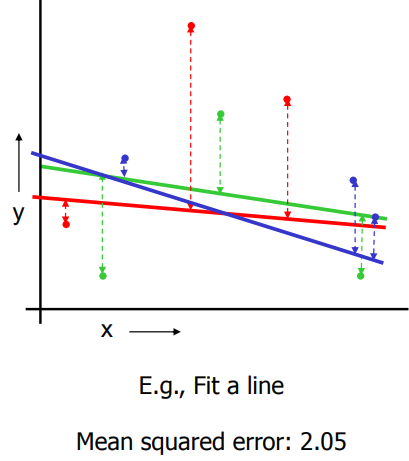
\includegraphics[width=0.3\linewidth]{images/img_20260324_102443.png}
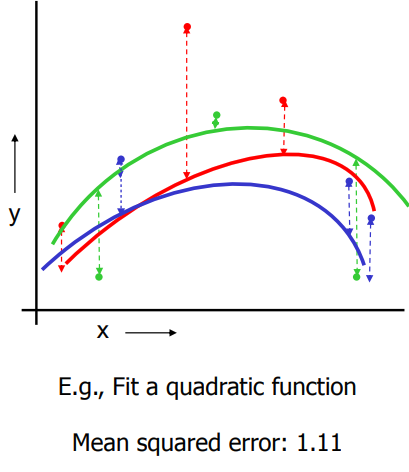
\includegraphics[width=0.3\linewidth]{images/img_20260324_102454.png}
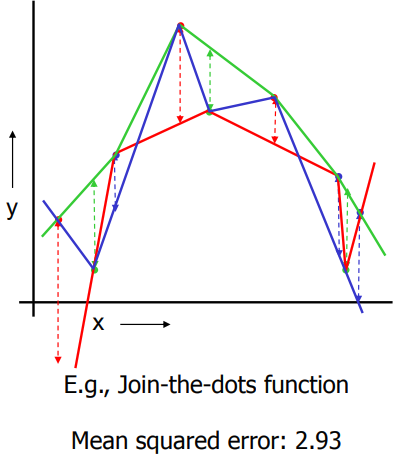
\includegraphics[width=0.3\linewidth]{images/img_20260324_102515.png}

\subsubsection{Which kind of cross-validation?}
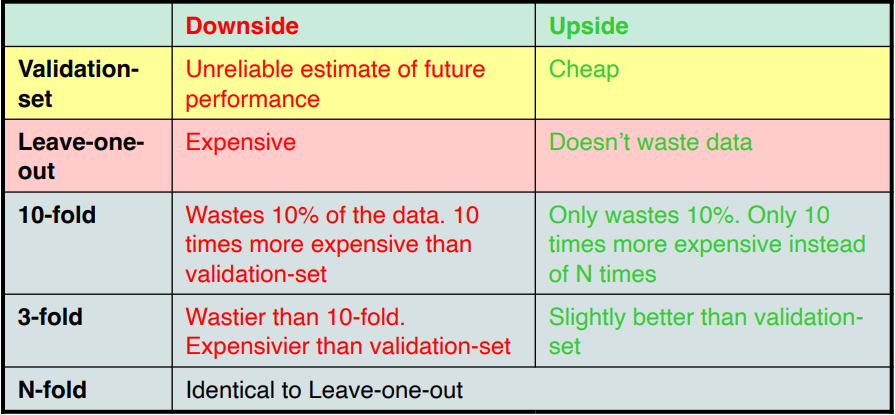
\includegraphics[width=0.55\linewidth]{images/img_20260324_102656.png}

To resume, cross-validation can help to:
\begin{itemize}
  \item Select the best model among a small number of candidates, but impractical with too many. 
  \item Find the best values for one hyper-parameter (e.g, $k$ in kNN), for this, one treats each value of the hyper-parameter as a separate model.
\end{itemize}

\subsection{Overfitting with a linear model}
Because the linear model is simple, overfitting occurs fairly rarely. 

Nevertheless, if there are fewer training samples than input
dimensions ($N\leq D + 1$), then one can always fit a
hyperplane that passes exactly through the training samples (overfitted model), it can occur for example when using feature expansion.

\subsubsection{Penalizing overfitting}
Thus to avoid this problem of overfitting, we will penalize overfitting by adding a regularizer to the empirical risk. 

This leads to a new training objective function of the form \[
E(w) = R(w) + \lambda E_w(w)
\]
where $R(w)$ is the empirical risk, $E_w(w)$ the regularizer, $\lambda$ is a hyper-parameter that defines the influence of the regularizer ($\lambda > 0$). So know we want not only to 
minimize the error on the data but to keep the weight as low as possible too. By adding this constraints, it reduces the complexity of overfitted model by making them simpler (the higher the hyperparameter $\lambda$, the stronger is the constraint, i.e., $\lambda = 1'000'000$ force the weights to be almost zero and results on a flat line ($\hat{y} \approx 0$)).
\subsubsection{Regularized linear regression}
One of the most common regularizers is the sum of squares
of the weights (there is a probabilistic motivation behind it) \[
  E_w(w) = w^Tw
\]
This lets us write regularized linear regression as \[
  min_w \sum_{i=1}^{N}(\phi(x_i)^Tw- y_i)^2 + \lambda w^Tw
\]
This remains a convex function (for $\lambda \geq 0$) and so we can still find the solution by zeroing out the gradient. 

We have \[ 
  \nabla E = \nabla R + \nabla E_w = 2 \sum_{i=1}^{N}\phi(x_i)(\phi(x_i)^Tw - y_i) + 2 \lambda w 
\]
Setting the gradient to zero yields \[
  \left(\sum_{i=1}^{N}\phi(x_i)\phi(x_i)^T + \lambda I_F\right)w^* = \sum_{i=1}^{N}\phi(x_i)y_i 
\]
where $I_F$ is the $F \times F$ identity matrix. 

Grouping the inputs in a matrix $\Phi$ and the outputs in a vector $y$, as before, gives the final solution \[
  w^* = (\Phi^T \Phi + \lambda I_F)^{-1}\Phi^T y
\]
Note that now we cannot use the pseudo-inverse anymore (as we add a regularizer). 

Regularized linear regression is also referred to \textit{as ridge
regression}.

Note that the regularizer affects the optimal value of the parameters, but \textbf{not}
the mathematical form of the prediction, which remains \[
  \hat{y} = (w*)^T \phi(x)
\]

\subsubsection{Multi-output ridge regression}
When dealing with multiple output dimensions, the
parameters are expressed in matrix form. 

We can then write multi-output ridge regression as \[
min_w \sum_{i=1}^{N}\left\|W^T \phi(x_i) - y_i\right\|^2 + \lambda \left\|W\right\|_F^2 
\]
where $\left\|W\right\|_F^2$ is the square Frobenius norm, equivalent to the sum of the square of all values in the matrix \textbf{W}.

By zeroing out the gradient we obtain the solution \[
  W^* = \left(\Phi^T \Phi + \lambda I_F\right)^{-1} \Phi^T Y
\]
Where \textbf{Y} is an $N \times C$ matrix (with $C$ output dimensions)

\subsubsection{Regularization on logistic regression}
Regularization may also be added to the cross-entropy loss used to train the logistic regression model. 

With a convex regularizer, such as the sum of squares, the overall
regularized risk remains convex. 

In fact, some implementation of the logistic regression has a regularizer by default (i.e : scikit-learn).

\subsubsection{Regularization and SVM}
As the SVM training proble is expressed as \[
\min_{w^{(0)}, \tilde{w}} \frac{1}{2C} \lVert \tilde{w} \rVert^2 
+ \sum_{i=1}^{N} \max \left(0,\, 1 - y_i \cdot \left(w^{(0)} + \tilde{w}^T x_i \right)\right)
\]

Minimizing $\left\|\tilde{w}\right\|^2$ (corresponds to the inverse of the margin (distance between the
decision boundary and the nearest sample)) is equivalent to maximizing the margin, which already acts as a built-in regularizer !
